% Chapter Template

\chapter{Planificació temporal} % Main chapter title

\label{Planificacio} % Change X to a consecutive number; for referencing this chapter elsewhere, use \ref{ChapterX}

El projecte està delimitat temporalment entre el mes de febrer del 2017 i el
mes de juny del 2017. L’assignatura GEP dona el tret de sortida al TFG ja
que els lliuraments d’aquesta assignatura són parts de la memòria final del
projecte. El projecte s’inicia el dia 13 de febrer i s’acaba a finals de juny amb la presentació oral. No obstant es marca una data límit prèvia a la presentació per tal d’assegurar que el projecte tingui una certa maduresa el dia de la defensa, aquest dia és el 15 de juny.

\section{Descripció de les tasques}

S’ha dividit la feina en tres grans fases. Per cadascuna d’elles s’explica quines tasques es duen a terme i les hores de dedicació previstes.

\begin{itemize}
\item{}\textbf{Fase inicial}\\
En la fase inicial del projecte és bàsic determinar que es vol construir.
Aquesta part del desenvolupament del projecte està marcada per la gestió del mateix. Es defineix clarament quin és l’abast, el problema que es
vol solucionar, l’estat actual de l’art, la metodologia a seguir, la planificació i la gestió econòmica.\\

En aquesta fase inicial també es dur a terme l’anàlisi de requisits del sistema, aquest punt es força important ja que és bàsic definir què ha de
satisfer l’aplicació per tal de considerar-la completa.\\

El projecte segueix la metodologia àgil Scrum, per tant, la definició del
backlog determinarà les històries d’usuari que s’han d’implementar per
tal de dur a terme el projecte. Una història d’usuari és una característica o funcionalitat de la plataforma independent a la resta, i per tant, el backlog és el conjunt ordenat d’aquestes característiques o funcionalitats. Quan es defineix una història d’usuari també s’hi afegeixen els criteris d’acceptació, que són unes condicions que ha de satisfer el sistema per tal de donar la història per acabada. El criteri que es fa servir per ordenar el backlog és la importància de la pròpia història i a l’hora de la selecció de les històries a desenvolupar durant una iteració concreta es mira l’ordre però també el tamany de la història. El tamany de la història ve definit pels punts d’història.\\

Durant aquesta fase es preveu un treball diari de 3 hores.

\item{}\textbf{Iteracions}\\
Una iteració es un període de temps durant el qual s’ha de desenvolupar
un conjunt d’històries d’usuari prèviament seleccionades. És important
que es desenvolupin de manera vertical, és a dir, en acabar una iteració
s’ha de tenir software que funcioni i, a més, integrat al que s’havia desenvolupat en la iteració anterior.\\

En l’inici de cada iteració es seleccionen les històries d’usuari que es volen desenvolupar i es crea un tauler utilitzant l’eina Trello. A mesura que es van completant aquestes histories es fan proves per veure que tot funcioni i es donen per acabades. El dia que acaba la iteració es valora la feina feta i es redefineix la velocitat (punts d’historia per iteració).
Durant el desenvolupament del projecte es duran a terme 5 iteracions distribuides en les següents dates:
\begin{itemize}
\item{}Iteració 1: 29 de març - 12 d’abril
\item{}Iteració 2: 13 d’abril - 26 d’abril
\item{}Iteració 3: 27 d’abril - 10 de maig
\item{}Iteració 4: 11 de maig - 24 de maig
\item{}Iteració 5: 25 de maig - 7 de juny
\end{itemize}
Durant aquesta fase del projecte es preveu un treball de 4 hores al dia.
\item{}\textbf{Fase final}\\
En la fase final del projecte es dedicaran tots els esforços en la redacció de
la memòria del projecte i la preparació de la presentació final. A més, es
duran a terme proves de l’aplicació amb la participació d’usuaris reals.
Aquesta fase es comença el dia 8 de juny i finalitza el dia 16 de juny amb
la previsió d’un treball diari de 3 hores.

\end{itemize}

\section{Diagrama de Gantt}

Per tal de definir bé la planificació del projecte s’utilitza un diagrama de Gantt (figura 3.2) i una taula explicativa (figura 3.1).

\begin{figure}[!h]
\centering
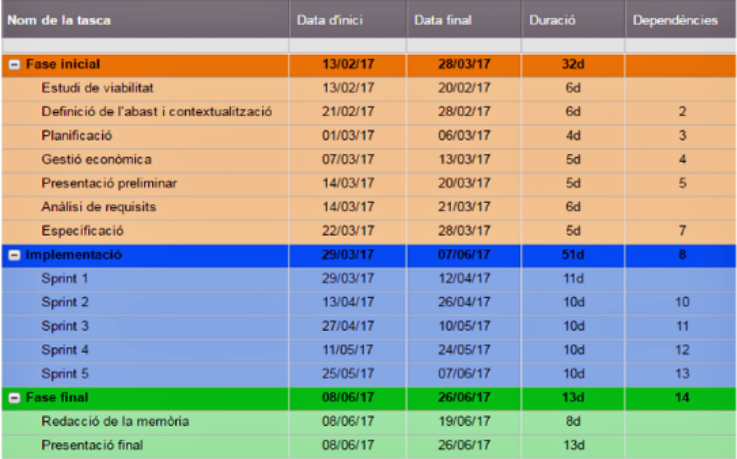
\includegraphics[scale=0.65]{Figures/planificacio.jpg}
\caption{Planificació del projecte.}
\end{figure}

\begin{figure}[!h]
\centering
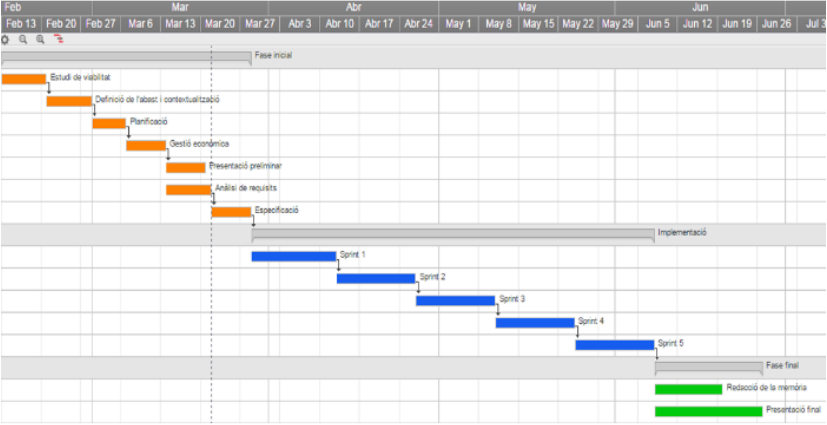
\includegraphics[scale=0.65]{Figures/Gantt.jpg}
\caption{Diagrama de Gantt.}
\end{figure}

\section{Recursos humans}

\begin{itemize}

\item{}\textbf{Cap de projecte:} Encarregat de la planificació i supervisió de les tasques a desenvolupar en un projecte així com de l’organització, coordinació i mediació de l’equip de recursos humans.
\item{}\textbf{Analista:} Estudia els problemas actuals per proposar una solución òptima i d’acord als recursos disponibles. Proporcionen les funcionalitats que tindrà el sistema mitjançant el model de casos d’ús.
\item{}\textbf{Dissenyador:} En base a la documentació proporcionada pels analistes, s’estructura i es defineix una arquitectura pel sistema que s’ha de desenvolupar. 
\item{}\textbf{Programador:} S’encarrega d’implementar el disseny proposat pels dissenyadors d’una forma eficient.
\item{}\textbf{Tester:} Prova el sistema per tal de detectar errors o recomanar modificacions, ha de redactar un informe després de cada prova efectuada.
\end{itemize}

\clearpage

\section{Recursos tècnics}

\newcolumntype{L}{>{\centering}m{4cm}}
\newcolumntype{M}{m{4cm}}
\newcolumntype{T}{m{12cm}}

\newcommand\tab[1][0.75cm]{\hspace*{#1}}

\begin{table}[!h]
\begin{tabular}{|M|L|M|}
\hline
\textbf{Recurs}& Tipus & Finalitat  \\ \hline
Recurs
Ordinador portàtil
Packard Bell i7, 4 GB
de Ram i windows 7
64x & Eina de desenvolupament & Desenvolupar l’aplicació i la memòria \\ \hline
Motorola Moto G amb Android 5.0 & Eina de desenvolupament &
Dur a terme les proves
durant el desenvolupament de l’aplicació \\ \hline
Android Studio v2.2.1 &
Eina de desenvolupament &
Desenvolupar l’aplicació mòbil. \\ \hline
Microsoft Office word
2007
Microsoft Office Power
Point 2007 & Eina de desenvolupament & Redacció d’informes \\ \hline
Point 2007
Adobe Photoshop 9 & Eina de desenvolupament & Edició i maquetació de
la presentació final. \\\hline
Adobe Reader XI & Eina de desenvolupament & Visualització de documents\\\hline
Correu electrònic
Gmail & Eina de comunicació & Comunicació amb la tutora del projecte\\\hline
Git & Eina de desenvolupament & Control de versions del codi font de l’aplicació \\\hline
LateX & Eina de desenvolupament & Redacció de la memòria final \\\hline
\end{tabular}
\label{}
\caption{Recursos tècnics}
\end{table}

\section{Valoració d'alternatives i pla d'acció}

Durant el desenvolupament del projecte poden sorgir desviacions de dos tipus:
\begin{itemize}

\item{}\textbf{Errors en la planificació}\\
Resulta força complicat ser precís en la planificació del projecte ja que és un equip completament nou en aquesta disciplina.\\

L’error pot venir donat per una planificació massa pessimista, en aquest
cas no hi hauria cap problema ja que durant les iteracions es podrien agafar més històries d’usuari seguint l’ordre del backlog. Acabar el projecte abans d’hora no seria perjudicial.\\

D’altra banda, l’error pot ser causat per una planificació massa optimis-
ta. En aquest cas si que és un problema ja que significa que l’equip no
pot acabar la feina a temps. Per afrontar aquesta situació s’ha reservat un
període d’una setmana abans de l’entrega final del projecte que es podria
utilitzar per acabar les històries pendents. A més, durant l’última iteració s’estudiaria l’opció de realitzar hores extra, i en el cas que no es pugui dur a terme tot el projecte es deixarien sense implementar les últimes històries del backlog ja que sempre són les menys prioritàries.\\

Tot i aquestes possibles desviacions degut a una mala planificació a cada final d’iteració i reunió amb la tutora s’evaluarà la situació i tenint en
compte les dates marcades es reafirmarà la planificació establerta o es fa-
ran les modificacions necessàries.

\item{}\textbf{Imprevistos}\\
Durant el desenvolupament del projecte poden sorgir imprevistos que
sigui quin sigui l’origen d’aquestes es solucionaran fent hores extra i prioritzant les tasques que aportin més valor al projecte.

\end{itemize}

